\documentclass[t,aspectratio=169]{beamer} % 使用16:9宽高比
\usetheme{Madrid} % 选择Madrid主题
\usecolortheme{default} % 使用默认颜色主题

% 设置字体
\usepackage[UTF8]{ctex}
\usefonttheme{structurebold} % 加粗结构字体

% 数学包
\usepackage{amsmath, amssymb, bm}
\usepackage{url}
\usepackage{booktabs}

% 图形包
\usepackage{graphicx}

% 标题页信息
\title[10.6.风格迁移]{第10章：卷积网络}
\subtitle{第6节：风格迁移 (Style Transfer)}
\author{《深度学习基础》课程小组}
% \institute{上海立信会计金融学院}
\date{\today}

\begin{document}

% 标题页
\frame{\titlepage}

% 目录页
\begin{frame}
    \frametitle{目录}
    \tableofcontents
\end{frame}

% ============================================================
% 第一部分：基本思想
% ============================================================
\section{基本思想}

\begin{frame}
    \frametitle{1. 神经风格迁移 (Neural Style Transfer)}
    \begin{itemize}
        \item 深度卷积网络中：
        \begin{itemize}
            \item \alert{早期层}：检测简单特征（边缘、纹理）
            \item \alert{后期层}：检测复杂实体（物体）
        \end{itemize}
        \item 利用这一性质：将一张图像以\alert{另一张图像的风格}重新渲染。
        \item 称为\alert{神经风格迁移} (Gatys, Ecker, and Bethge, 2015)。
    \end{itemize}
    \begin{figure}
        \centering
        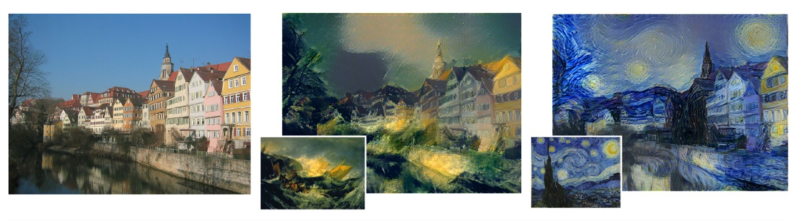
\includegraphics[width=0.65\textwidth]{figure-10-32.png}
        \caption{运河场景照片以 Turner 和 van Gogh 风格重新渲染。}
    \end{figure}
\end{frame}

\begin{frame}
    \frametitle{1.1 目标与误差函数}
    \begin{itemize}
        \item 生成合成图像 $\mathbf{G}$：
        \begin{itemize}
            \item \alert{内容}由图像 $\mathbf{C}$ 定义
            \item \alert{风格}取自图像 $\mathbf{S}$
        \end{itemize}
        \item 误差函数为两项之和：
        \begin{equation}
            E(\mathbf{G}) = E_{\text{content}}(\mathbf{G}, \mathbf{C}) + E_{\text{style}}(\mathbf{G}, \mathbf{S})
            \tag{10.13}
        \end{equation}
        \item 内容和风格的概念由这两项的\alert{泛函形式隐式定义}。
        \item 从\alert{随机初始化}图像开始，用\alert{梯度下降}最小化 $E(\mathbf{G})$。
    \end{itemize}
\end{frame}

% ============================================================
% 第二部分：内容误差
% ============================================================
\section{内容误差}

\begin{frame}
    \frametitle{2. 内容误差 $E_{\text{content}}$}
    \begin{itemize}
        \item 选择网络中的一个\alert{特定卷积层}。
        \item 测量图像 $\mathbf{G}$ 和 $\mathbf{C}$ 作为输入时，该层单元的\alert{预激活值}。
        \item 用\alert{平方和误差}鼓励相应的预激活值相似：
        \begin{equation}
            E_{\text{content}}(\mathbf{G}, \mathbf{C}) = \sum_{i,j,k} \{a_{ijk}(\mathbf{G}) - a_{ijk}(\mathbf{C})\}^2
            \tag{10.14}
        \end{equation}
        \item $a_{ijk}(\mathbf{G})$：输入 $\mathbf{G}$ 时，通道 $k$ 位置 $(i,j)$ 的预激活值。
        \item \textbf{选择哪一层影响结果}：
        \begin{itemize}
            \item \alert{较早层}：匹配边缘等低层特征
            \item \alert{较晚层}：匹配更复杂结构甚至完整物体
        \end{itemize}
        \item 内容误差要求\alert{位置匹配}：$\mathbf{G}$ 与 $\mathbf{C}$ 在相同位置具有相似预激活值。
    \end{itemize}
\end{frame}

% ============================================================
% 第三部分：风格误差
% ============================================================
\section{风格误差}

\begin{frame}
    \frametitle{3. 风格误差 $E_{\text{style}}$}
    \begin{itemize}
        \item \textbf{直觉}：风格由卷积层内\alert{不同通道特征的共现}决定。
        \item 例：风格图像中垂直边缘通常与橙色斑块关联 $\Rightarrow$ 生成图像 $\mathbf{G}$ 也应如此。
        \item \textbf{与内容误差的关键区别}：
        \begin{itemize}
            \item 内容误差：\alert{位置匹配}
            \item 风格误差：\alert{位置无关}，可来自任意位置
            \item 因此对特征图中的位置\alert{取平均}
        \end{itemize}
    \end{itemize}
    \begin{block}{风格矩阵（Gram 矩阵）}
        度量通道 $k$ 与 $k'$ 特征共现程度：
        \begin{equation}
            F_{kk'}(\mathbf{G}) = \sum_{i=1}^{I} \sum_{j=1}^{J} a_{ijk}(\mathbf{G})a_{ijk'}(\mathbf{G})
            \tag{10.15}
        \end{equation}
        $K$ 个通道 $\Rightarrow$ $K \times K$ 矩阵，称为\alert{风格矩阵}。
    \end{block}
\end{frame}

\begin{frame}
    \frametitle{3.1 风格误差的定义}
    比较图像 $\mathbf{G}$ 和 $\mathbf{S}$ 的风格矩阵：
    \begin{equation}
        E_{\text{style}}(\mathbf{G}, \mathbf{S}) = \frac{1}{(2IJK)^2} \sum_{k=1}^{K} \sum_{k'=1}^{K} \{F_{kk'}(\mathbf{G}) - F_{kk'}(\mathbf{S})\}^2
        \tag{10.16}
    \end{equation}
    \begin{itemize}
        \item $F_{kk'}$：风格矩阵元素
        \item $I, J$：特征图维度
        \item $K$：通道数
        \item 归一化因子 $\frac{1}{(2IJK)^2}$ 平衡不同层、不同尺寸特征图的误差量级
    \end{itemize}
\end{frame}

\begin{frame}
    \frametitle{3.2 多层风格贡献}
    使用\alert{多层}贡献获得更令人满意的结果：
    \begin{equation}
        E_{\text{style}}(\mathbf{G}, \mathbf{S}) = \sum_{l} \lambda_l E_{\text{style}}^{(l)}(\mathbf{G}, \mathbf{S})
        \tag{10.17}
    \end{equation}
    \begin{itemize}
        \item $l$：卷积层索引
        \item $\lambda_l$：决定不同层之间的\alert{相对权重}
        \item 同时也决定相对于\alert{内容误差项}的权重
        \item 这些权重系数通过\alert{主观判断经验性调整}
    \end{itemize}
    \begin{block}{不同层的影响}
        \begin{itemize}
            \item 浅层权重高 $\Rightarrow$ 风格更偏纹理和细节
            \item 深层权重高 $\Rightarrow$ 风格更偏结构和语义
        \end{itemize}
    \end{block}
\end{frame}

% ============================================================
% 第四部分：总结
% ============================================================
\section{总结}

\begin{frame}[allowframebreaks]
    \frametitle{4. 本节总结}
    \begin{itemize}
        \item \alert{神经风格迁移}：
        \begin{itemize}
            \item 利用 CNN 早期层检测简单特征、后期层检测复杂实体的性质
            \item 将一张图像以另一张图像的风格重新渲染
        \end{itemize}
        \item \alert{误差函数}：
        \begin{equation}
            E(\mathbf{G}) = E_{\text{content}}(\mathbf{G}, \mathbf{C}) + E_{\text{style}}(\mathbf{G}, \mathbf{S})
        \end{equation}
        \item \alert{内容误差}：
        \begin{itemize}
            \item 选择特定卷积层，比较 $\mathbf{G}$ 与 $\mathbf{C}$ 的预激活值
            \item 平方和误差
            \item 要求\alert{位置匹配}
            \item 浅层 $\to$ 低层特征；深层 $\to$ 复杂结构
        \end{itemize}
        \item \alert{风格误差}：
        \begin{itemize}
            \item 风格由不同通道特征的\alert{共现}决定
            \item 风格矩阵（Gram 矩阵）$F_{kk'}$
            \item 对位置\alert{取平均}，位置无关
            \item 多层加权求和：$E_{\text{style}} = \sum_l \lambda_l E_{\text{style}}^{(l)}$
            \item $\lambda_l$ 经验性调整
        \end{itemize}
        \item 从随机初始化图像开始，用\alert{梯度下降}最小化 $E(\mathbf{G})$。
    \end{itemize}
\end{frame}

% ============================================================
% 第五部分：参考文献
% ============================================================
\section{参考文献}

\begin{frame}
    \frametitle{5. 参考文献}
    \begin{itemize}
        \item 教材：Bishop, C. M. \& Bishop, H. (2023). Deep Learning Foundations and Concepts. Springer Nature Switzerland AG.
        \item Gatys, L. A., Ecker, A. S., \& Bethge, M. (2015). A neural algorithm of artistic style.
    \end{itemize}
\end{frame}

\end{document}